% ============================================================================
% Downhill-Simplex-Algorithmus
% ============================================================================

\ifdefined\outputformat\else\def\outputformat{}\fi
\documentclass[\outputformat]{beamer}

\usetheme[
  pageofpages=von, % String used between the current and the total page count.
  alternativetitlepage=false, % Use the fancy title page.
  titlepagelogo=logo, % Logo for the first page.
]{Torino}

\usepackage[utf8x]{inputenc} % Schriftkodierung mit Umlauten
\usepackage[T1]{fontenc}
\usepackage[ngerman]{babel}
\usepackage{graphicx} % Grafiken
\usepackage{tabularx}
\usepackage{booktabs}
\usepackage{textcomp}
\usepackage{amsmath}
\usepackage{pifont}

\usepackage{multirow} 

\usepackage{bm}
\usepackage{bbm}
\usepackage{color}
\usepackage{tikz}
\usetikzlibrary{arrows,shapes,snakes}

\usepackage{colortbl}

\graphicspath{{abbildungen/}}

%\beamersetuncovermixins{\opaqueness<1>{25}}{\opaqueness<2->{15}}
\logo{
\includegraphics[height=0.0625\paperheight]{HSR_Logo_CMYK.pdf}}

\author{Selina Malacarne \and\\ Raphael Nestler}
\title{Simplex Algorithmus für nichtlineare Optimierungsprobleme}
\subtitle{Simplex-Downhill Algorithmus}
%\institute{
\includegraphics[height=0.13\paperheight]{HSR_Logo_CMYK.pdf}}
\date{13. Mai 2013}

\setcounter{tocdepth}{1}

% ============================================================================
\begin{document}

\begin{frame}
\titlepage
\end{frame}

\begin{frame}{Programm}
\tableofcontents
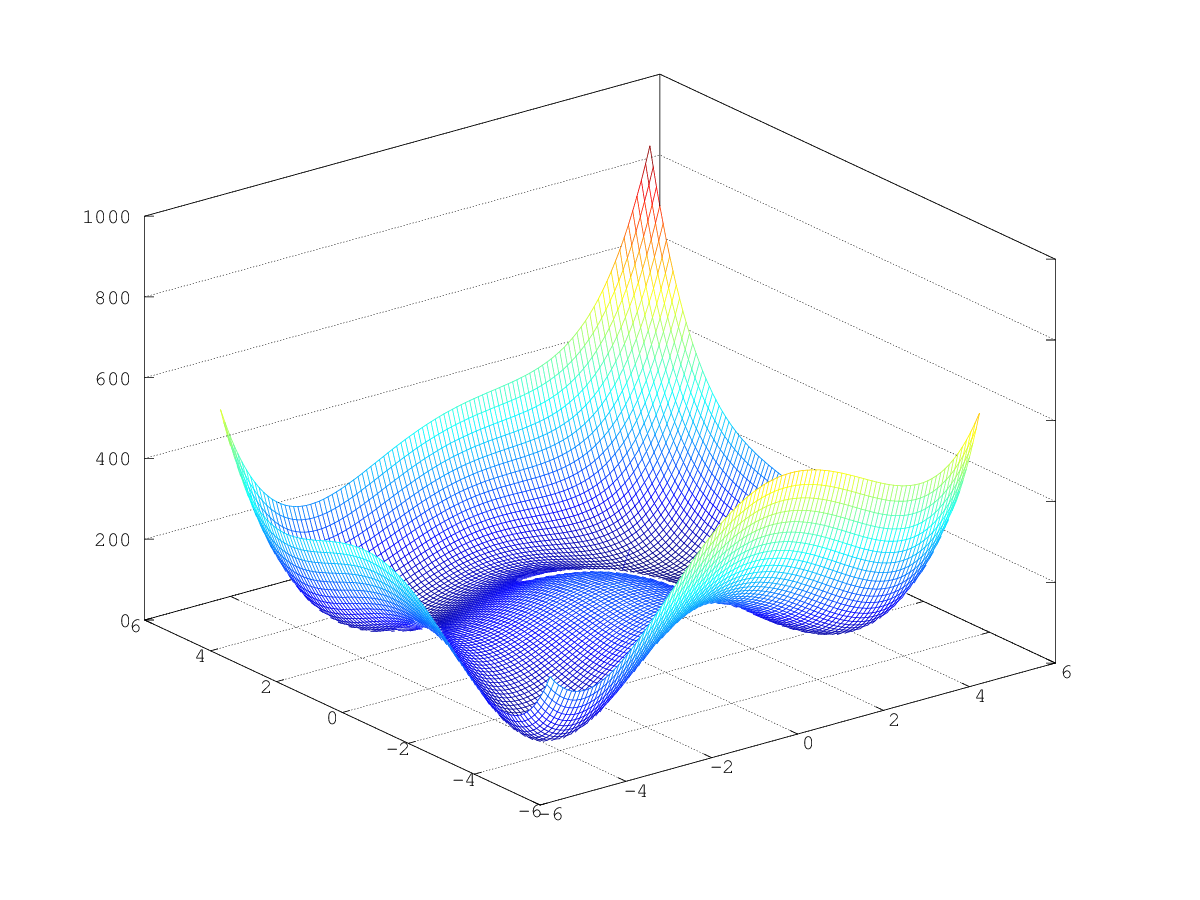
\includegraphics[height=0.5\paperheight]{himmelblau.png}
\end{frame}

% ============================================================================
\section{Einleitung} 
\begin{frame}{Programm}\tableofcontents[currentsection]\end{frame}

\begin{frame}{Grundlagen}
\begin{itemize}
	\item Beschrieben von John Nelder und Roger Mead ($\approx 1965$)
	\item \textbf{NICHT} verwechseln mit Simplex Algorithmus
	\item Anwendung: 
	\begin{itemize}
		\item Optimierung nichtlinearer Funktionen mit mehreren Parametern 
		\item Kurvenfitten (bspw. Messwerte an Kurve angleichen)
	\end{itemize}	
	\item Kategorie: Hillclimbing- oder Downhill Suchverfahren
\end{itemize}
\end{frame}

\begin{frame}{Merkmale}
\begin{itemize}
	\item Vergleicht mehrere Punkte (N-Dimensionen+1)
	\item Verwendung von \textbf{einfachst möglichen Volumina} (Simplex $\rightarrow$ bei n=2: Simplex = Dreieck)
	\item Vorteile
	\begin{itemize}
		\item Benötigt \textbf{keine} Ableitungen
		\item Einfach und robust
	\end{itemize}
	\item Nachteile
	\begin{itemize}
		\item Langsam (konvergiert linear)
		\item Kann in lokales Minima fallen
	\end{itemize} 
\end{itemize}
\end{frame}

% ============================================================================
\section{Der Algorithmus} 
\begin{frame}{Programm}\tableofcontents[currentsection]\end{frame}

\begin{frame}{Übersicht}
\newcommand{\highlight}{white}

%\usetikzlibrary{arrows}
\begin{tikzpicture}[node distance = 1.7cm,every node/.style={rectangle,fill=white},
  block/.style={draw},
  highlight/.style={draw,fill=\highlight},
  line/.style = {draw,-latex'}
]

\node (start) [block] {N+1 Startpunkte $x_i$ wählen (Simplex bilden)};

\node (a1) [block, below of=start] { $y_i = f(x_i)$ berechnen};

\node (a2) [block, below of=a1] { Bestes ($y_{min}$) und schlechtestes ($y_{max}$) $y_i$ bestimmen};

\node (a3) [block, below of=a2 ]{$y_{min}$ gut genug?};

\node (ende) [block, below of=a3] {Ende};

\node (a4) [highlight, left of=a3, node distance=6cm] {Neuer Simplex bilden};



\path[line] (start) -- (a1);
\path[line] (a1) -> (a2);
\path[line] (a2) -> (a3);

\path[line] (a3) -> node{ja} (ende);
\path[line] (a3) -> node{nein} (a4);

\path[line] (a4)  |-  (a1.west);

\end{tikzpicture}

\end{frame}
\begin{frame}{Übersicht}
\newcommand{\highlight}{green}

%\usetikzlibrary{arrows}
\begin{tikzpicture}[node distance = 1.7cm,every node/.style={rectangle,fill=white},
  block/.style={draw},
  highlight/.style={draw,fill=\highlight},
  line/.style = {draw,-latex'}
]

\node (start) [block] {N+1 Startpunkte $x_i$ wählen (Simplex bilden)};

\node (a1) [block, below of=start] { $y_i = f(x_i)$ berechnen};

\node (a2) [block, below of=a1] { Bestes ($y_{min}$) und schlechtestes ($y_{max}$) $y_i$ bestimmen};

\node (a3) [block, below of=a2 ]{$y_{min}$ gut genug?};

\node (ende) [block, below of=a3] {Ende};

\node (a4) [highlight, left of=a3, node distance=6cm] {Neuer Simplex bilden};



\path[line] (start) -- (a1);
\path[line] (a1) -> (a2);
\path[line] (a2) -> (a3);

\path[line] (a3) -> node{ja} (ende);
\path[line] (a3) -> node{nein} (a4);

\path[line] (a4)  |-  (a1.west);

\end{tikzpicture}

\end{frame}

\begin{frame}{Neuer Simplex bilden}
Vier mögliche Varianten
\begin{enumerate}
\item Reflexion
\item Expansion
\item Kontraktion 1/2
\item Komprimierung
\end{enumerate}
\end{frame}

\begin{frame}{Reflexion / Expansion}

\usetikzlibrary{arrows}

\definecolor{uuuuuu}{rgb}{0.27,0.27,0.27}
\definecolor{zzttqq}{rgb}{0.6,0.2,0}
\definecolor{qqqqff}{rgb}{0,0,1}
\begin{tikzpicture}[line cap=round,line join=round,>=triangle 45,x=1.0cm,y=1.0cm]
\clip(4.5,0.26) rectangle (12.32,4.94);
\fill[color=zzttqq,fill=zzttqq,fill opacity=0.1] (5.74,3.1) -- (10.36,3.92) -- (11,1.7) -- cycle;
\draw [color=zzttqq] (5.74,3.1)-- (10.36,3.92);
\draw [color=zzttqq] (10.36,3.92)-- (11,1.7);
\draw [color=zzttqq] (11,1.7)-- (5.74,3.1);
\draw (9.03,2.91)-- (7.71,1.89);
\draw (7.71,1.89)-- (6.91,1.29);
\begin{scriptsize}
\fill [color=qqqqff] (5.74,3.1) circle (1.5pt);
\draw[color=qqqqff] (5.78,3.48) node {$x_{min}$};
\fill [color=qqqqff] (10.36,3.92) circle (1.5pt);
\draw[color=qqqqff] (10.96,4.18) node {$x_{max}$};
\fill [color=qqqqff] (11,1.7) circle (1.5pt);
\draw[color=qqqqff] (11.28,1.96) node {$x_3$};
\fill [color=uuuuuu] (9.03,2.91) circle (1.5pt);
\draw[color=uuuuuu] (9.34,3.16) node {$x_m$};
\fill [color=qqqqff] (7.71,1.89) circle (1.5pt);
\draw[color=qqqqff] (8.52,1.74) node {$x_{ref}$};
\fill [color=uuuuuu] (6.91,1.29) circle (1.5pt);
\draw[color=uuuuuu] (7.66,1.08) node {$x_{streck}$};
\end{scriptsize}
\end{tikzpicture}

\end{frame}

\begin{frame}{Kontraktion 1}

\usetikzlibrary{arrows}

\definecolor{uuuuuu}{rgb}{0.27,0.27,0.27}
\definecolor{zzttqq}{rgb}{0.6,0.2,0}
\definecolor{qqqqff}{rgb}{0,0,1}
\begin{tikzpicture}[line cap=round,line join=round,>=triangle 45,x=1.0cm,y=1.0cm]
\clip(4.6,0.68) rectangle (12.12,5);
\fill[color=zzttqq,fill=zzttqq,fill opacity=0.1] (5.74,2.92) -- (10.36,3.74) -- (11,1.52) -- cycle;
\draw [color=zzttqq] (5.74,2.92)-- (10.36,3.74);
\draw [color=zzttqq] (10.36,3.74)-- (11,1.52);
\draw [color=zzttqq] (11,1.52)-- (5.74,2.92);
\draw (10.36,3.74)-- (9.03,2.73);
\begin{scriptsize}
\fill [color=qqqqff] (5.74,2.92) circle (1.5pt);
\draw[color=qqqqff] (5.78,3.3) node {$x_{min}$};
\fill [color=qqqqff] (10.36,3.74) circle (1.5pt);
\draw[color=qqqqff] (10.96,4) node {$x_{max}$};
\fill [color=qqqqff] (11,1.52) circle (1.5pt);
\draw[color=qqqqff] (11.28,1.78) node {$x_3$};
\fill [color=uuuuuu] (9.03,2.73) circle (1.5pt);
\draw[color=uuuuuu] (9.44,2.62) node {$x_m$};
\fill [color=uuuuuu] (9.7,3.23) circle (1.5pt);
\draw[color=uuuuuu] (10.38,3.12) node {$x_{kon}$};
\end{scriptsize}
\end{tikzpicture}

\end{frame}

\begin{frame}{Kontraktion 2}

\usetikzlibrary{arrows}

\definecolor{uuuuuu}{rgb}{0.27,0.27,0.27}
\definecolor{zzttqq}{rgb}{0.6,0.2,0}
\definecolor{qqqqff}{rgb}{0,0,1}
\begin{tikzpicture}[line cap=round,line join=round,>=triangle 45,x=1.0cm,y=1.0cm]
\clip(3.88,0.38) rectangle (12.6,5.2);
\fill[color=zzttqq,fill=zzttqq,fill opacity=0.1] (5.74,2.92) -- (10.36,3.74) -- (11,1.52) -- cycle;
\draw [color=zzttqq] (5.74,2.92)-- (10.36,3.74);
\draw [color=zzttqq] (10.36,3.74)-- (11,1.52);
\draw [color=zzttqq] (11,1.52)-- (5.74,2.92);
\draw (9.03,2.73)-- (7.71,1.71);
\begin{scriptsize}
\fill [color=qqqqff] (5.74,2.92) circle (1.5pt);
\draw[color=qqqqff] (5.78,3.3) node {$x_{min}$};
\fill [color=qqqqff] (10.36,3.74) circle (1.5pt);
\draw[color=qqqqff] (10.96,4) node {$x_{max}$};
\fill [color=qqqqff] (11,1.52) circle (1.5pt);
\draw[color=qqqqff] (11.28,1.78) node {$x_3$};
\fill [color=uuuuuu] (9.03,2.73) circle (1.5pt);
\draw[color=uuuuuu] (9.44,2.62) node {$x_m$};
\fill [color=qqqqff] (7.71,1.71) circle (1.5pt);
\draw[color=qqqqff] (8.52,1.56) node {$x_{ref}$};
\fill [color=uuuuuu] (8.37,2.22) circle (1.5pt);
\draw[color=uuuuuu] (9.0,2.25) node {$x_{kon2}$};
\end{scriptsize}
\end{tikzpicture}
\end{frame}

\begin{frame}{Auswahl der Variante}
\resizebox{1\textwidth}{!}{
\usetikzlibrary{shapes}
\begin{tikzpicture}[
  top/.style={draw,align=center,text width=5cm},
  med/.style={draw,align=center,text width=5cm},
  fin/.style={ellipse,draw,align=center}
]

\tikzstyle{level 1}=[sibling distance=150mm,align=center]
\tikzstyle{level 2}=[sibling distance=100mm,align=center]
\tikzstyle{level 3}=[sibling distance=80mm]


\node (start) at (0,1.5)[top] {$x_{max}$ am Mittelpunkt des restlichen Simplex ($x_m$) spiegeln $\rightarrow$ $x_{ref}$};

\node[top](top){$y_{ref}$ besser als  $y_{min}$?}
	child { node {Ja} child {child { child  { child { child {
		node[med] {Expansion: In Richtung $y_{ref}$ mit Faktor $\gamma$ Strecken  $\rightarrow y_{streck} $}
		child{
			node[med]  {$y_{streck}$ besser als $y_{min}$?}
			child { node {ja}
			child { node [fin]{$x_{max}$ mit $x_{streck}$ ersetzen} }}
			child { node {nein}
			child { node(a2) [fin]{$x_{max}$ mit $x_{ref}$ ersetzen} }}
		}
	}}}}}}
	child {
		node {Nein}
		child  {
		node [med] {$y_{ref}$ besser als zweitschlechtestes $y_i$ ?}
		child { node (b1) [] {Ja} }
		child { node {Nein} 
		child { node[med] {Ist $y_{ref}$ besser als $y_{max}$? }
			child {node{Nein}
				child { node (kont)[med] {Kontraktion: Rücke mit Faktor $\beta$ näher an Mittelpunkt $\rightarrow y_{kon}$ }
					child { node[med]  {Ist $y_{kon}$ besser als $y_{max}$?}
						child {node {Ja}
							child {node[fin] {Ersetze $x_{max}$ durch $x_{kon}$}}
						}
						child {node {Nein}
							child {node[fin] {Komprimierung: Rücke alle $x_i$ zu $x_{min}$ } }
						}
					}
				}
			}
			child {node {Ja}
				child { node (zukont)[med] {Ersetze $x_{max}$ durch $x_{ref}$ } }
			}
		}
		}
	}
	}
;
\draw (zukont) -- (kont);
\draw (b1) -- (a2);
\draw (start) --(top);

\end{tikzpicture}
}

\end{frame}


% ============================================================================
\section{Beispiel}
\begin{frame}{Programm}\tableofcontents[currentsection]\end{frame}

\begin{frame}{Minimum der Quadratfunktion}

\end{frame}


\end{document}
